\chapter{Git e GitHub-CLI}
\par
\section{O que é o Git?}
O Git é um software open source, gratuito e multiplataforma voltado para o versionamento de código. Ele oferece um sistema de controle de versão distribuído, amplamente utilizado no desenvolvimento de software, que permite que múltiplos desenvolvedores trabalhem simultaneamente em um mesmo projeto. O Git rastreia as alterações realizadas nos arquivos, possibilitando reverter modificações, comparar versões e gerenciar ramificações (branches) de forma eficiente e segura.
\subsection{Instalação do Git}
\begin{enumerate}
  \item Abra o Prompt de Comando ou PowerShell.
  \item Digite o comando:
  \begin{verbatim}
    winget search git
  \end{verbatim}
  \item Na primeira vez que algum comando do Winget for executado, ele pedirá o aceite dos termos de uso. Ao aceitar, digitando \texttt{Y} ou \texttt{y}.
  \item Nesse comando \texttt{winget search git}, será buscado na base do winget todas as ocorrências em que o termo \texttt{git} aparece e será retornado uma tabela com os resultados associando o nome do programa, seu \textcolor{cyan}{id} para a instalação e algumas outras informações.
  \begin{figure}[H]
    \centering
    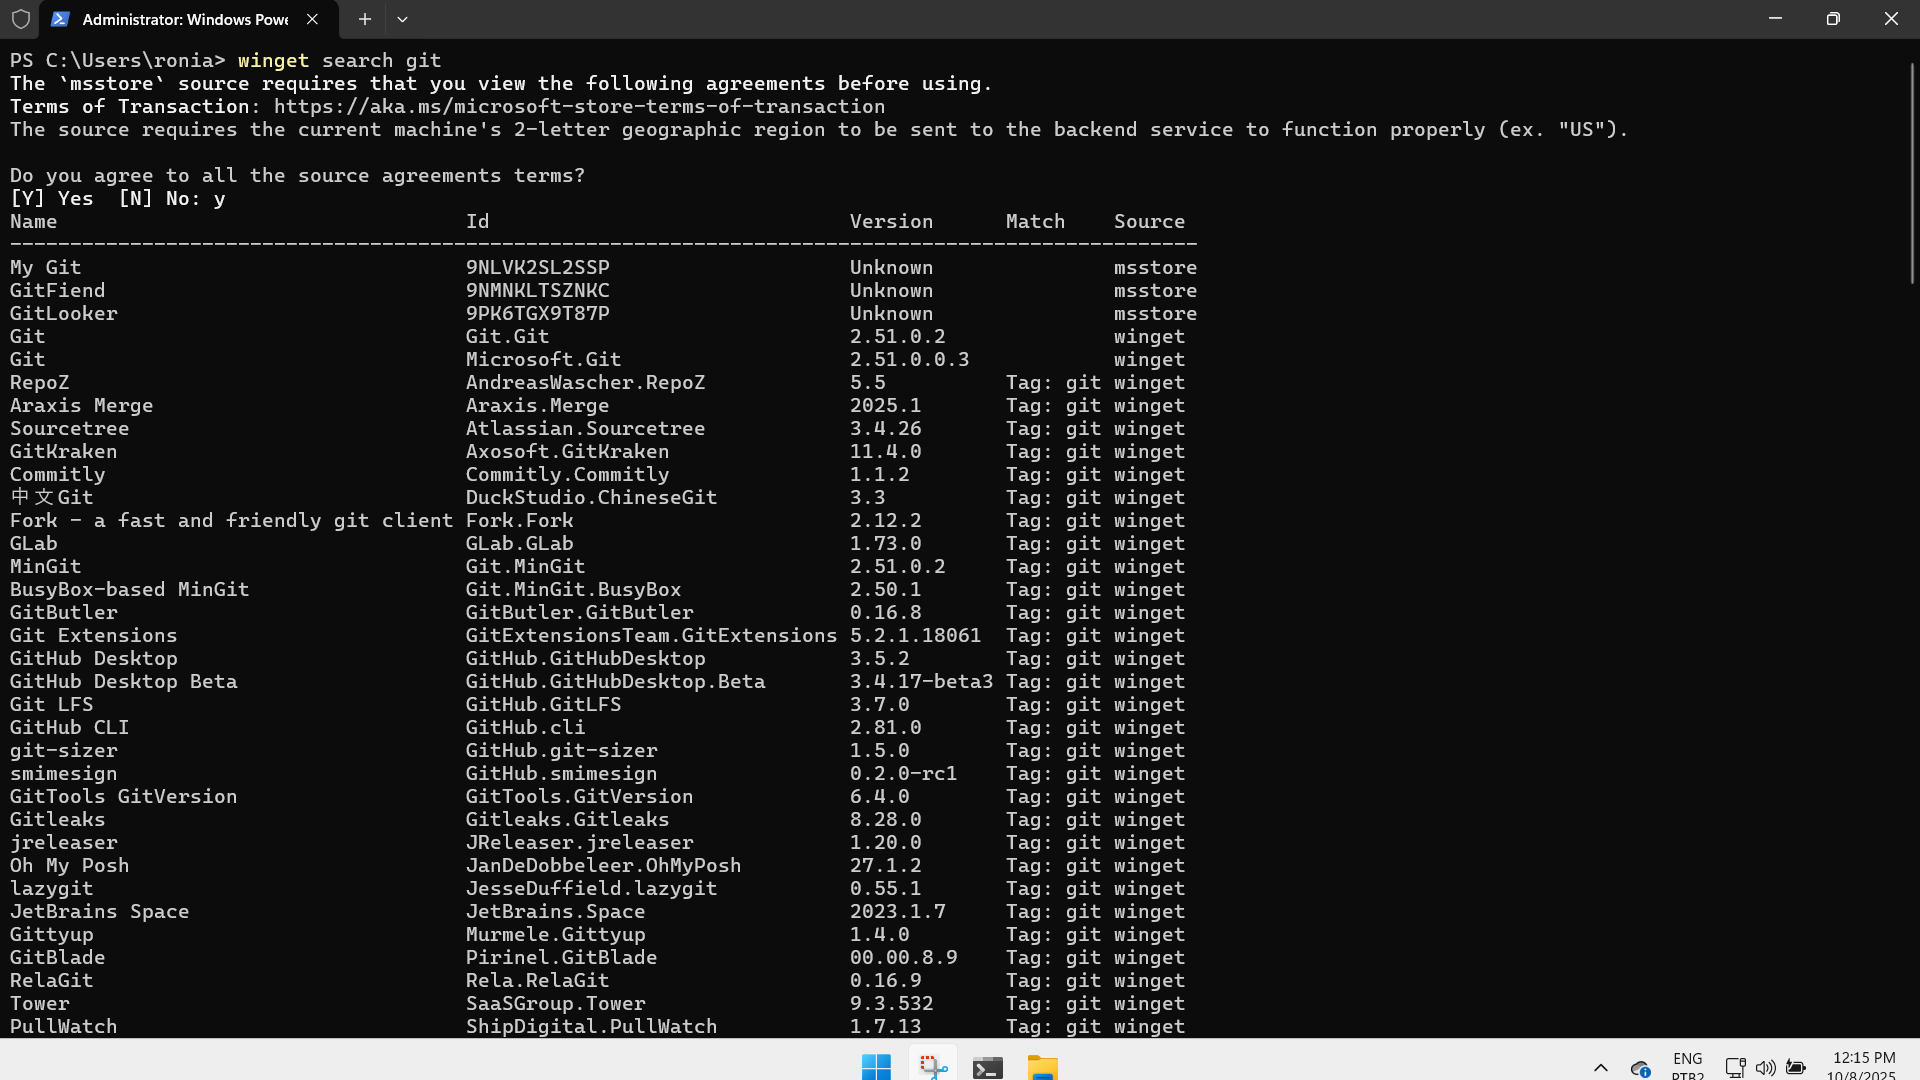
\includegraphics[width=0.9\textwidth]{./assets/images/08_winget_search.png}
    \caption{Buscando o Git no Winget.}
    \label{fig:winget_search}
  \end{figure} 
  \item Assim que localizar o software que deseja, copie ou memorize seu \textcolor{cyan}{id}, em nosso caso o \textcolor{cyan}{id} = \textcolor{cyan}{Git.Git}, e digite o comando:
  \begin{verbatim}
    winget install Git.Git
  \end{verbatim}
  e pressione Enter.
  \item Siga as instruções na tela para concluir a instalação.
  \item Aguarde a conclusão da instalação.
  \begin{figure}[H]
    \centering
    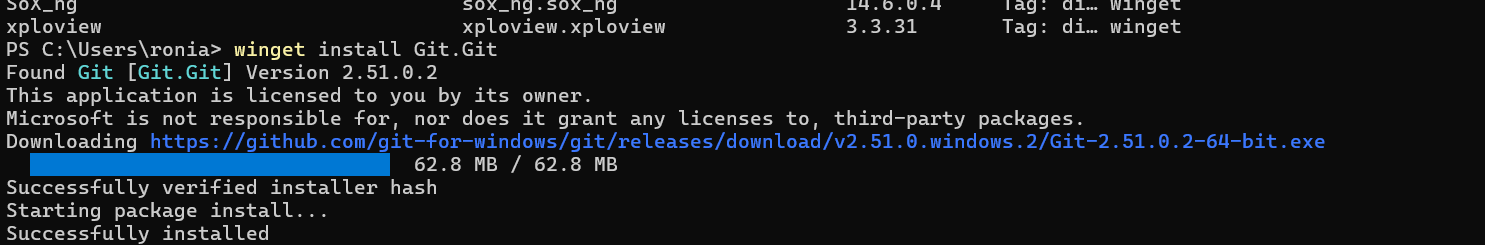
\includegraphics[width=0.9\textwidth]{./assets/images/09_install_git.png}
    \caption{Instalação do Git.}
    \label{fig:install_git}
  \end{figure}
  \item Verifique a instalação digitando, em alguns casos o Windows exige que o terminal seja reiniciado para que as variáveis de ambiente adicionadas com a instalação sejam carregadas corretamente:
  \begin{verbatim}
    git --version
  \end{verbatim}
  O comando deve retornar a versão do Git instalada.
  \begin{figure}[H]
    \centering
    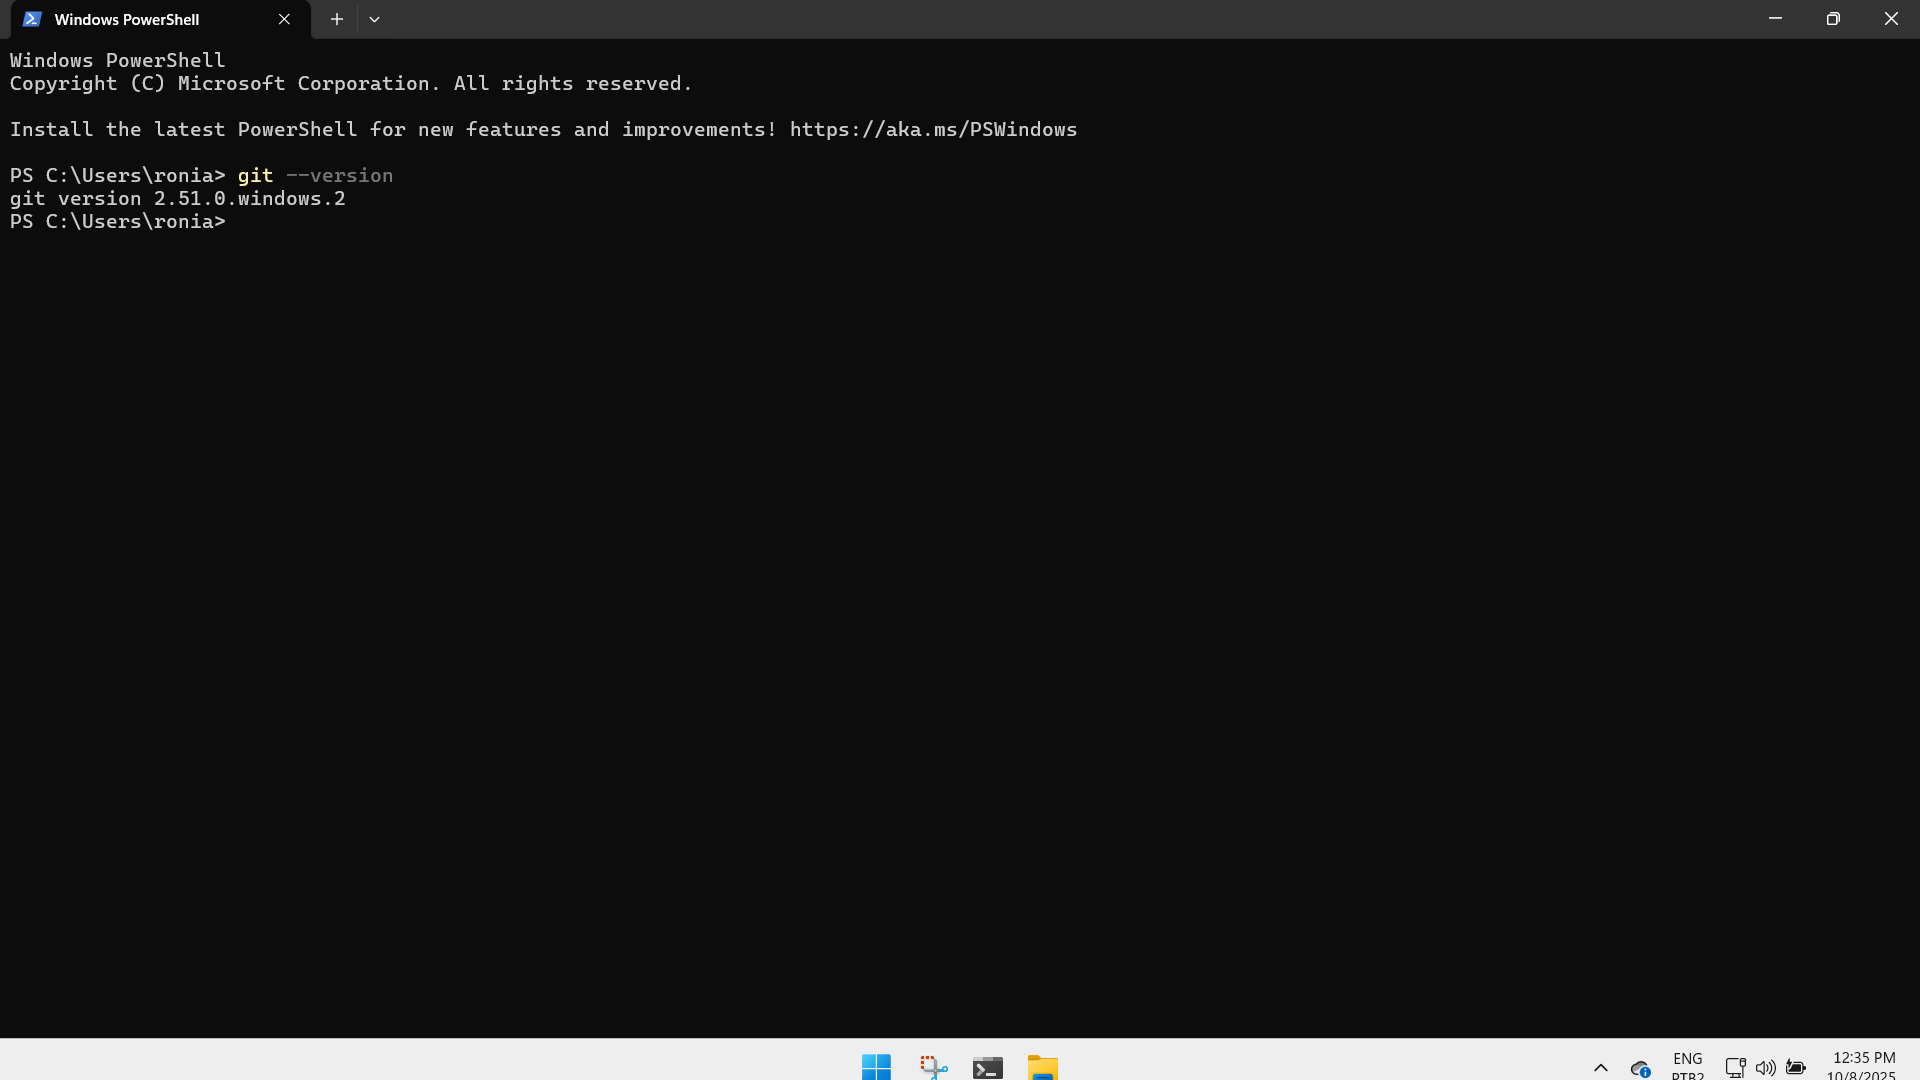
\includegraphics[width=0.9\textwidth]{./assets/images/10_git_version.png}
    \caption{Verificando se o Git está instalado.}
    \label{fig:git_version}
  \end{figure}
\end{enumerate}
\par
\section{O que é o GitHub-CLI?}
O GitHub-CLI (Command Line Interface) é uma ferramenta de linha de comando desenvolvida pela GitHub, Inc., que permite interagir com os repositórios e recursos do GitHub diretamente pelo terminal, sem a necessidade de acessar a interface web.

Com o GitHub-CLI, é possível executar operações comuns como clonar repositórios, criar issues, abrir e revisar pull requests, gerenciar branches, autenticar usuários, visualizar status de workflows e automatizar fluxos de trabalho, integrando-se perfeitamente com o Git e com scripts de automação.

Essa ferramenta é especialmente útil para desenvolvedores que preferem trabalhar no terminal, proporcionando agilidade, automação e maior produtividade no gerenciamento de projetos hospedados no GitHub.
\subsection{Instalação do GitHub-CLI}
\begin{enumerate}
  \item Abra o Prompt de Comando ou PowerShell.
  \item Agora \textcolor{cyan}{id} = \textcolor{cyan}{GitHub.cli}, e digite o comando:
  \begin{verbatim}
    winget install GitHub.cli
  \end{verbatim}
  e pressione Enter.
  \item Aguarde a conclusão da instalação.
  \begin{figure}[H]
    \centering
    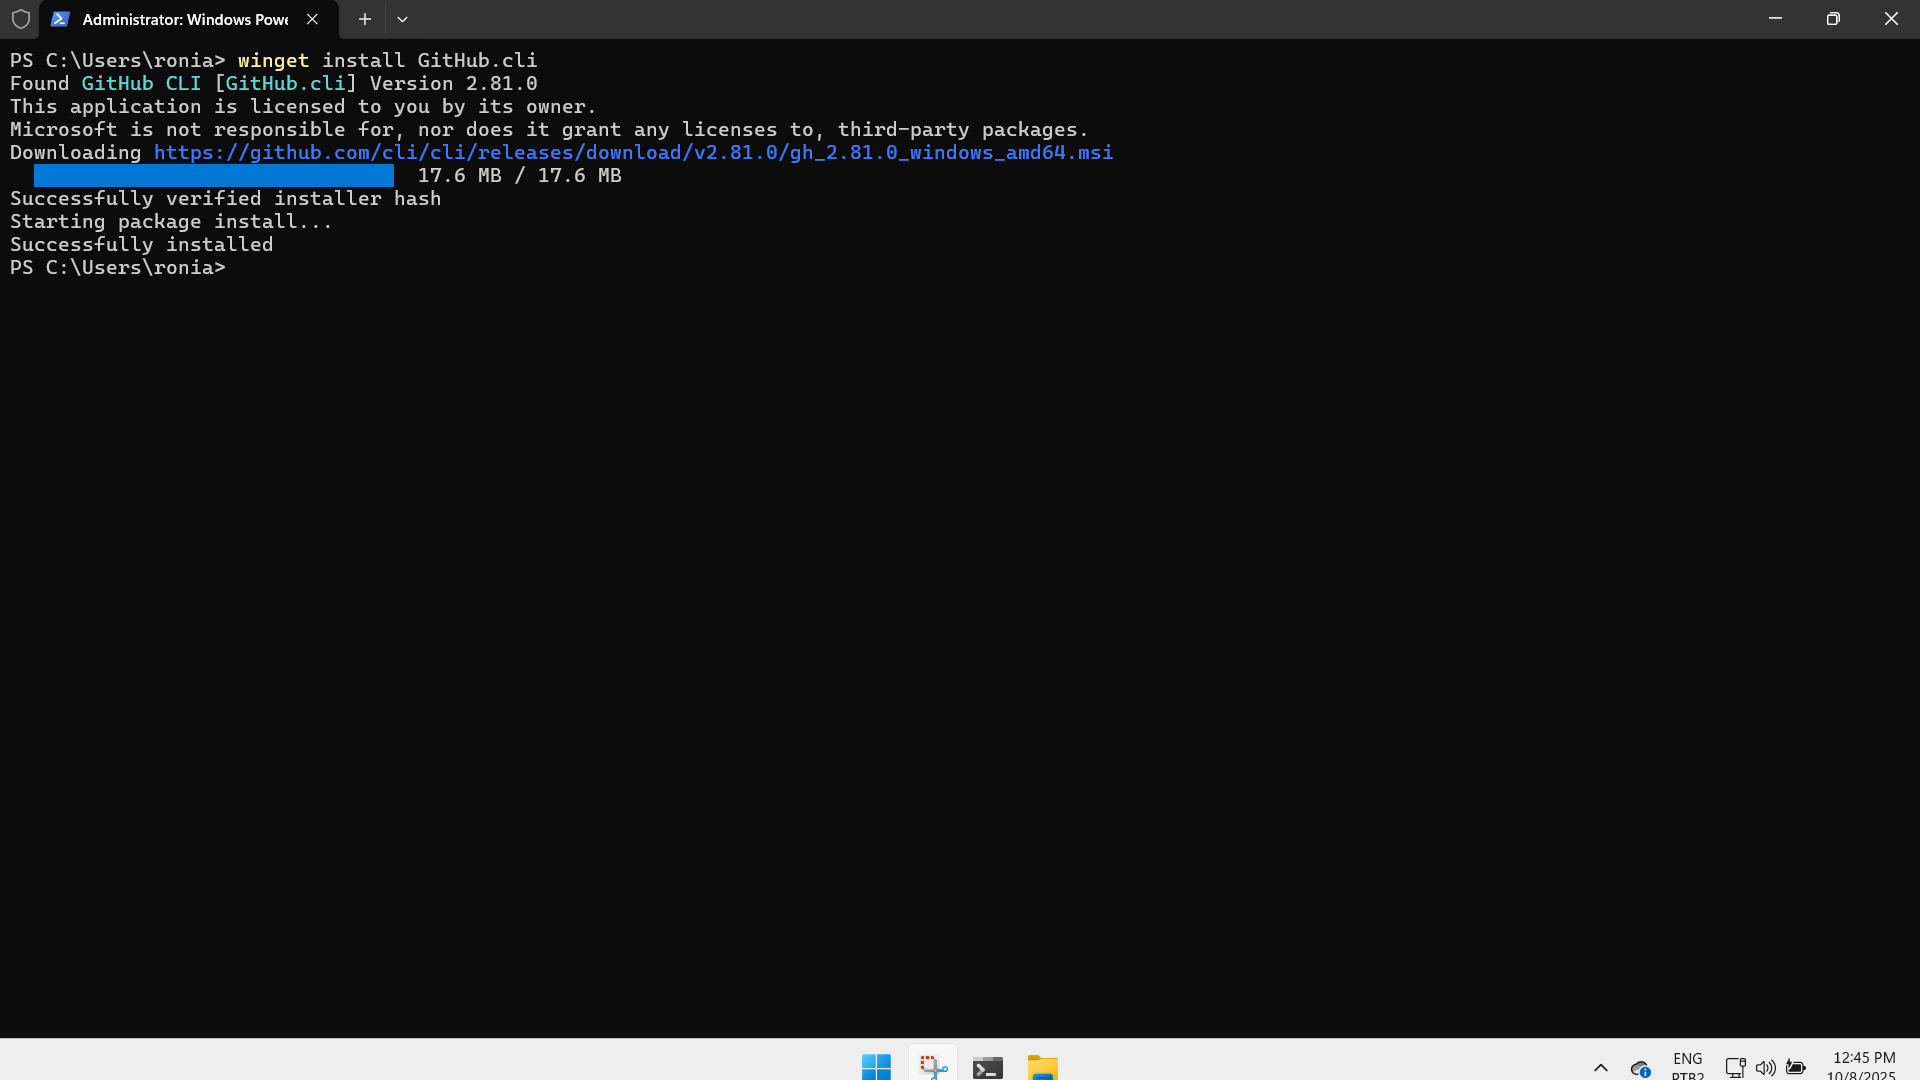
\includegraphics[width=0.9\textwidth]{./assets/images/11_install_cli.png}
    \caption{Instalando o GitHub-CLI.}
    \label{fig:install_cli}
  \end{figure}
  \item Verifique a instalação digitando:
  \begin{verbatim}
    gh --version
  \end{verbatim}
    O comando deve retornar a versão do GitHub-CLI instalada.
    \begin{figure}[H]
    \centering
    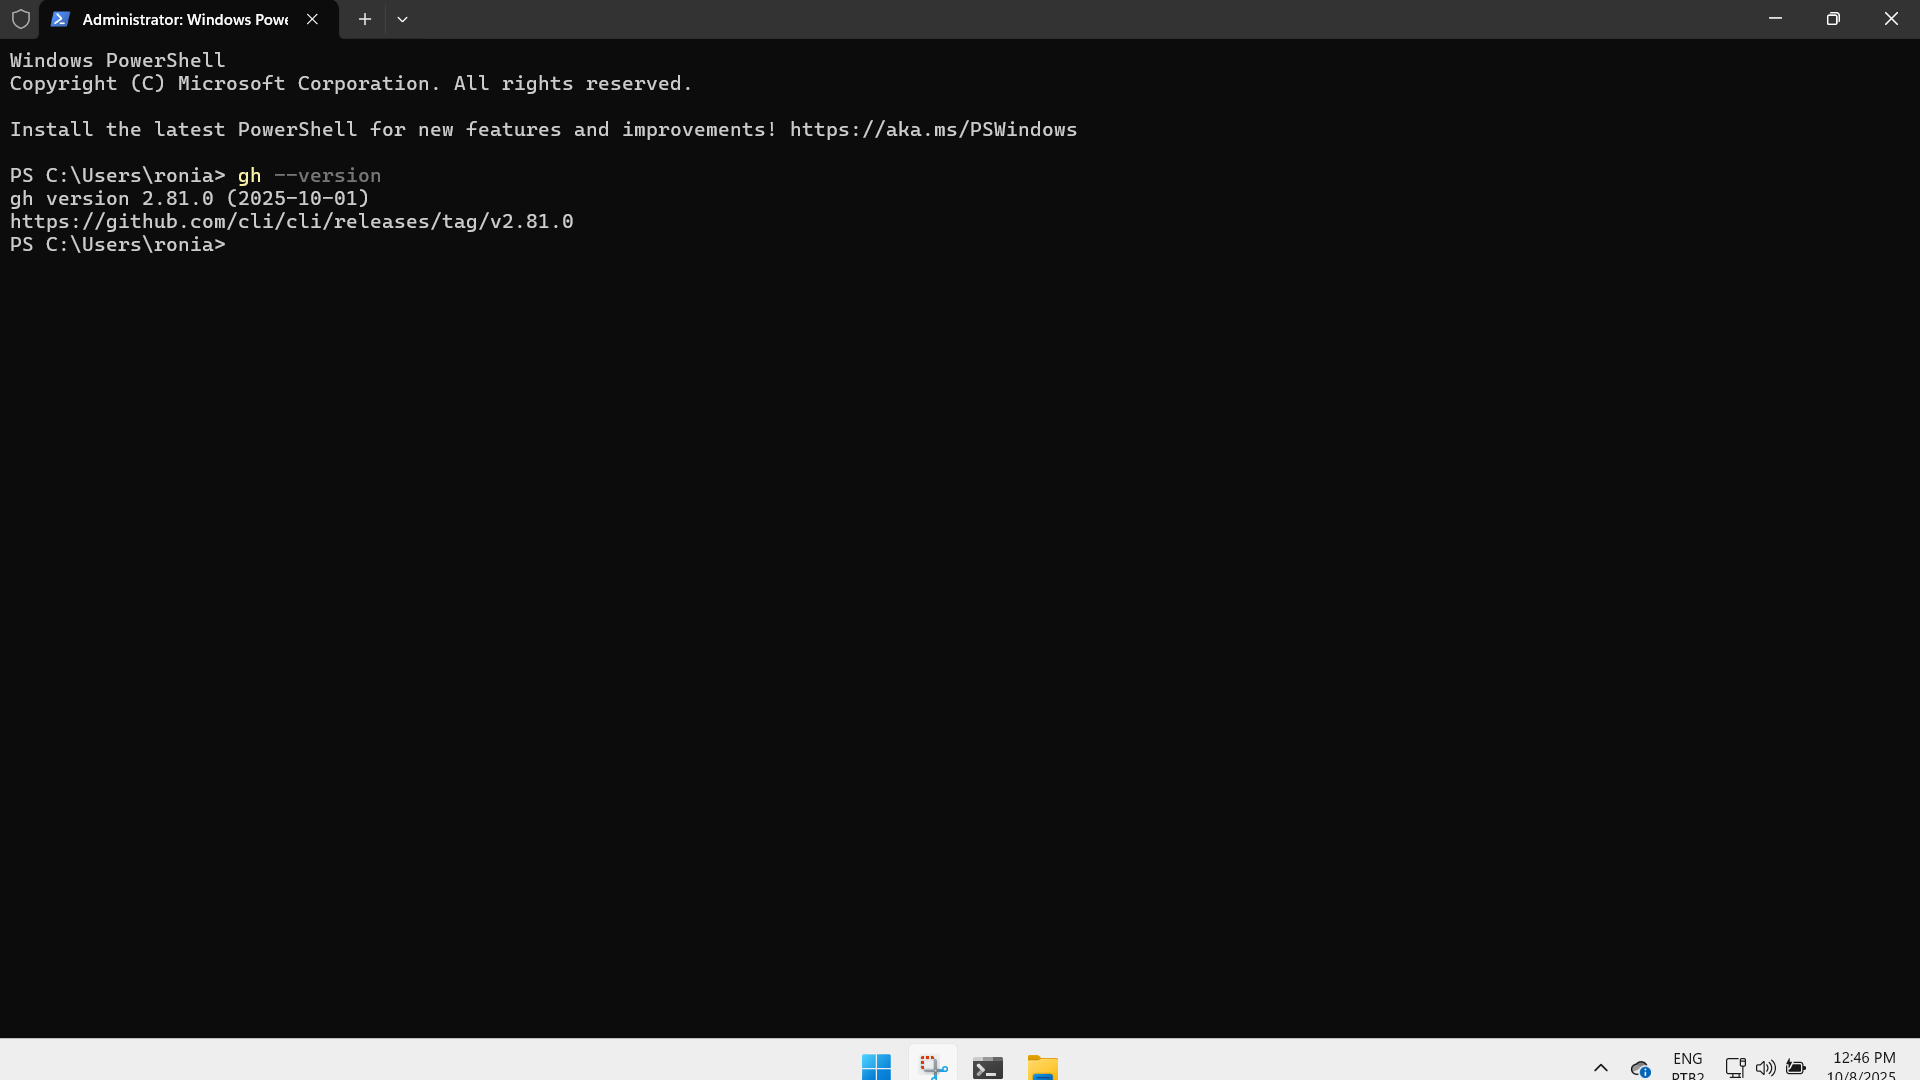
\includegraphics[width=0.9\textwidth]{./assets/images/12_cli_version.png}
    \caption{Verificando se o GitHub-CLI está instalado.}
    \label{fig:cli_version}
  \end{figure}
\end{enumerate}
\par
\section{Configuração do Git e GitHub-CLI}
Após a instalação do Git e do GitHub-CLI, é necessário realizar algumas configurações iniciais para garantir que suas informações estejam corretas ao fazer commits e interagir com o GitHub.
\par
\subsection{Autenticação}
Existem duas formas seguras de autenticação para o Git, a primeira envolve a geração de um token de acesso pessoal (PAT - Personal Access Token) no GitHub, que é usado como senha ao fazer push ou pull de repositórios remotos. A segunda forma é a autenticação via SSH, que envolve a criação de um par de chaves SSH (pública e privada) e a adição da chave pública à sua conta do GitHub. A autenticação via SSH é geralmente mais segura e conveniente, pois elimina a necessidade de inserir o token ou senha repetidamente.

OBS.: \textbf{Desde agosto de 2021, o GitHub não aceita mais autenticação via senha para operações Git que envolvem repositórios remotos. Portanto, é obrigatório o uso de tokens de acesso pessoal (PAT) ou autenticação via SSH para essas operações.}

A opção dois é usando o GitHub-CLI, que facilita o processo de autenticação. A seguir, estão os passos para configurar a autenticação usando o GitHub-CLI.
\par
\subsubsection{Autenticação com o GitHub-CLI}
Para autenticar-se no GitHub-CLI, execute o comando:
\begin{verbatim}
  gh auth login
\end{verbatim}
Siga as instruções na tela para concluir o processo de autenticação.
\begin{figure}[H]
  \centering
  \caption{Efetuando a autenticação com o GitHub-CLI - Passo 1.}
  \label{fig:gh_auth_login_0}
  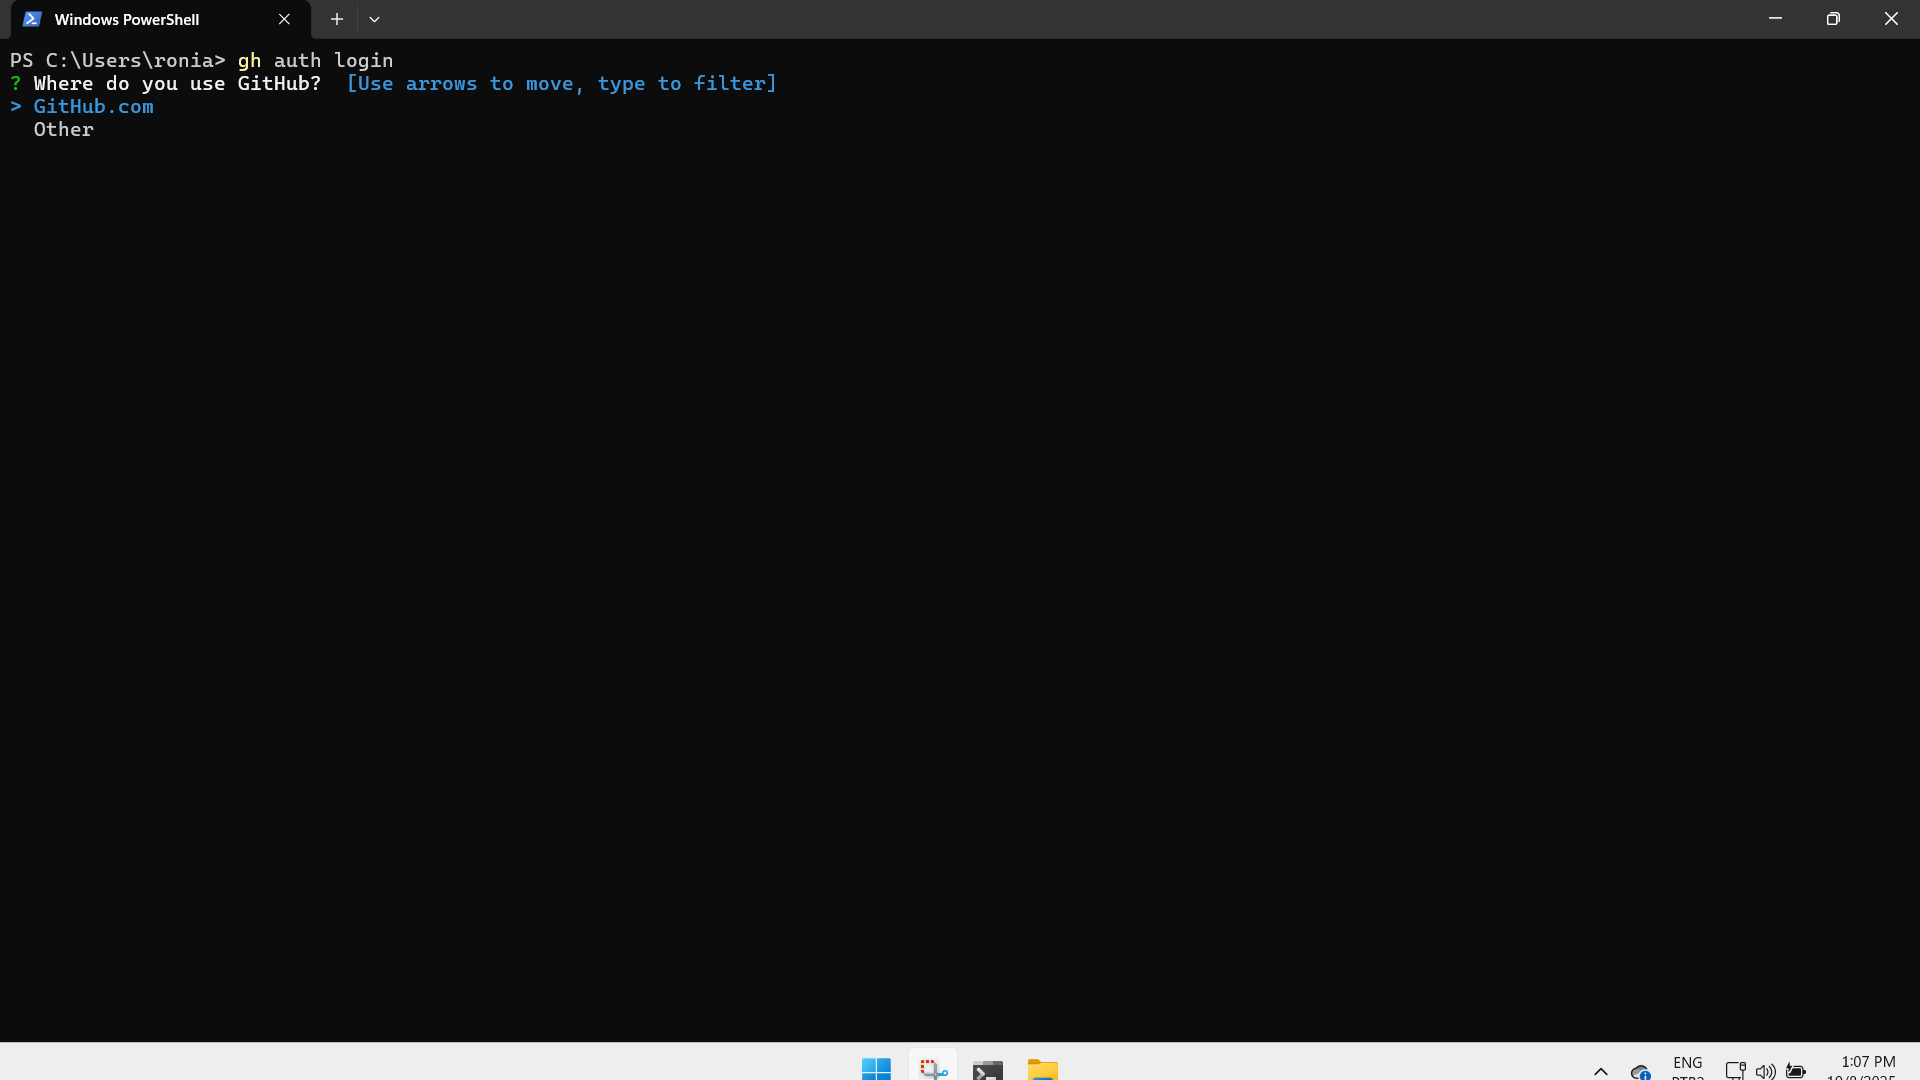
\includegraphics[width=0.9\textwidth]{./assets/images/13_0_gh_auth_login.png}
  \caption{Efetuando a autenticação com o GitHub-CLI - Passo 2.}
  \label{fig:gh_auth_login_1}
  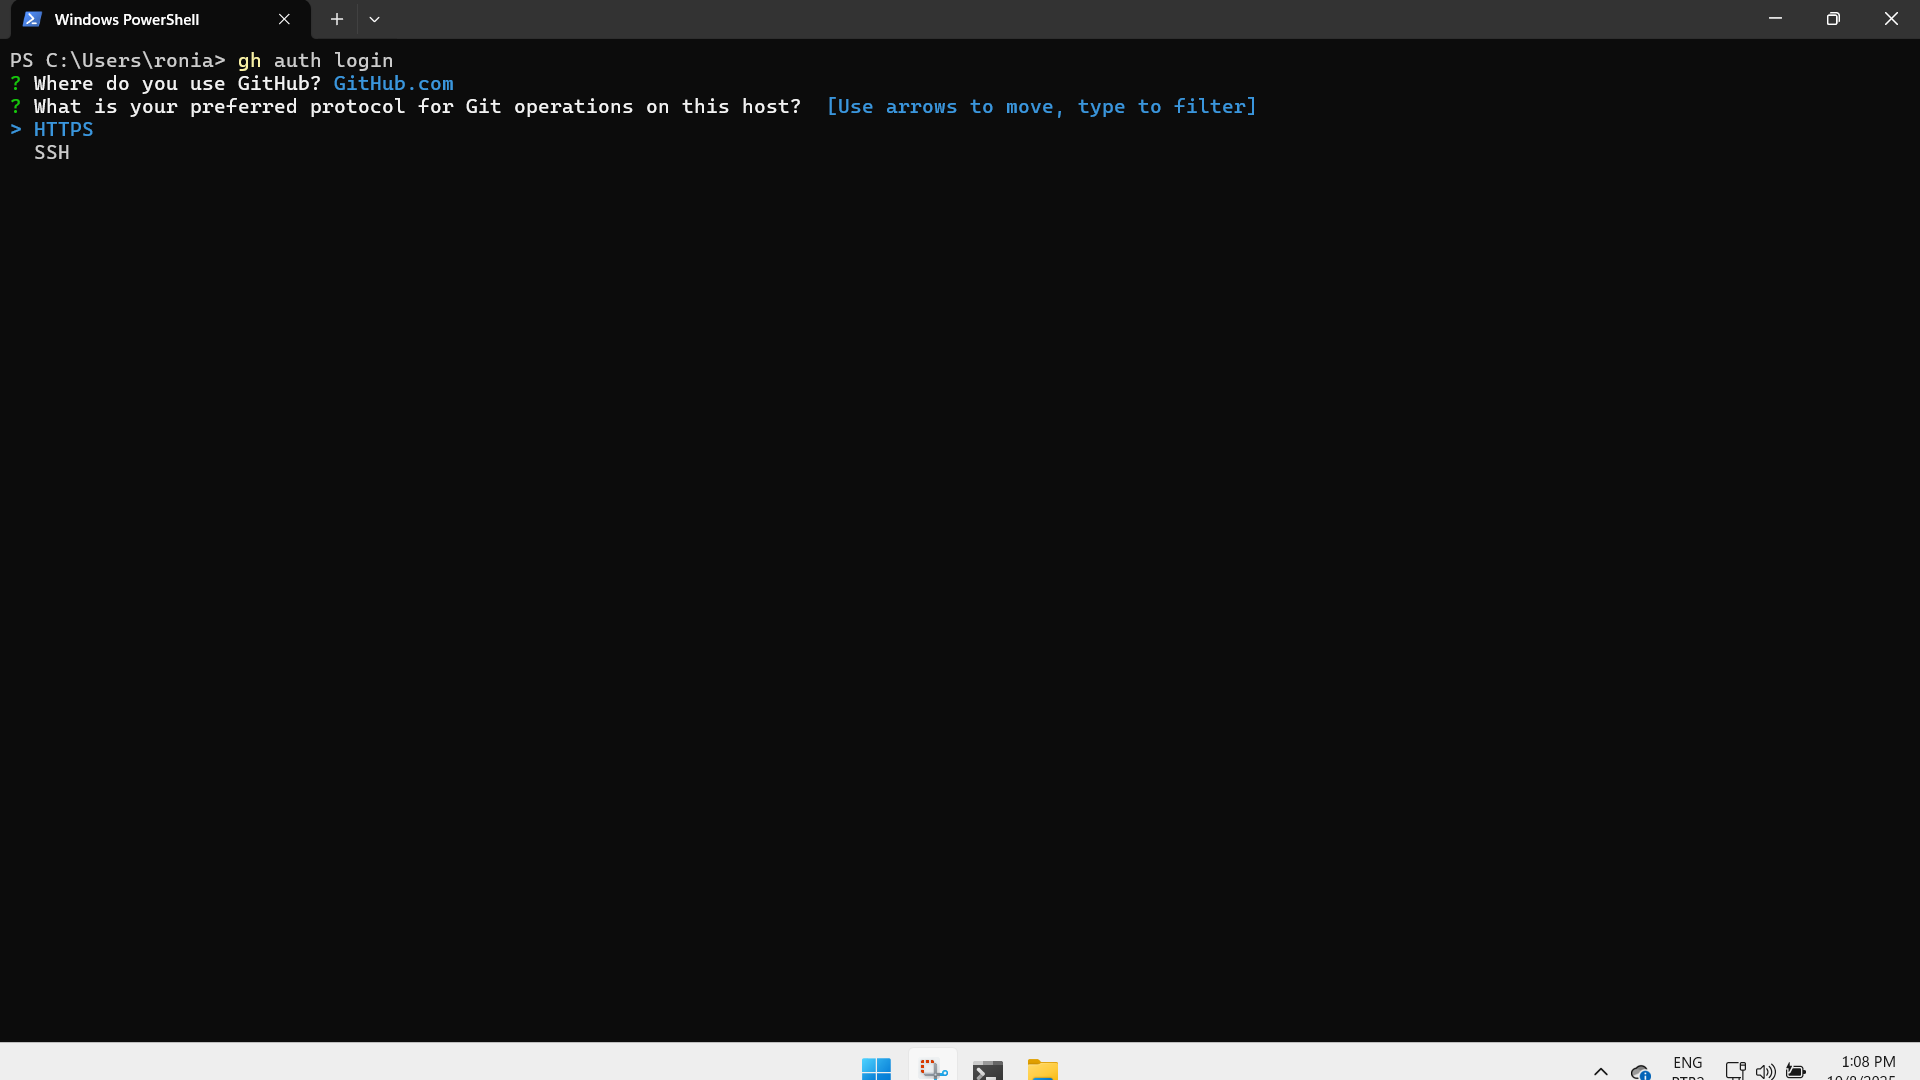
\includegraphics[width=0.9\textwidth]{./assets/images/13_1_gh_auth_login.png}
  \caption{Efetuando a autenticação com o GitHub-CLI - Passo 3.}
  \label{fig:gh_auth_login_2}
  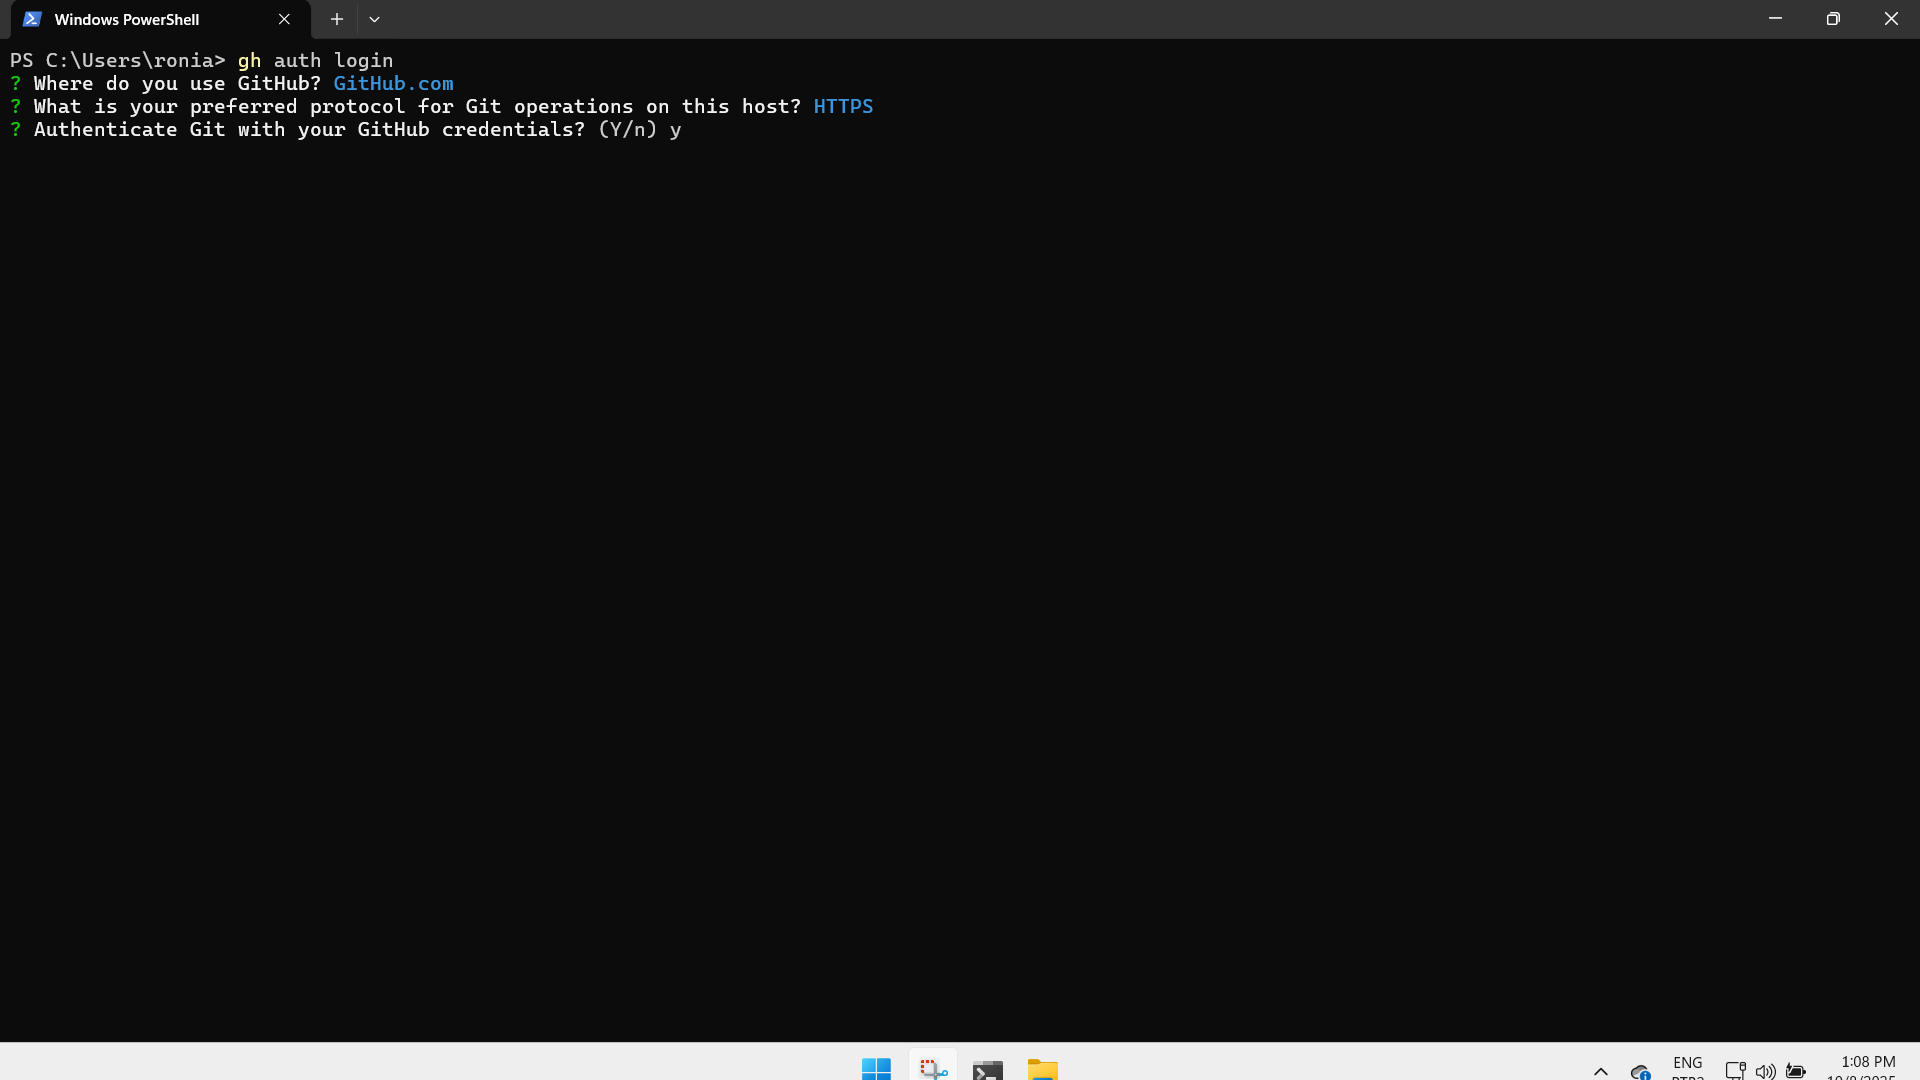
\includegraphics[width=0.9\textwidth]{./assets/images/13_2_gh_auth_login.png}
\end{figure}
\begin{figure}[H]
  \centering
  \caption{Efetuando a autenticação com o GitHub-CLI - Passo 4.}
  \label{fig:gh_auth_login_3}
  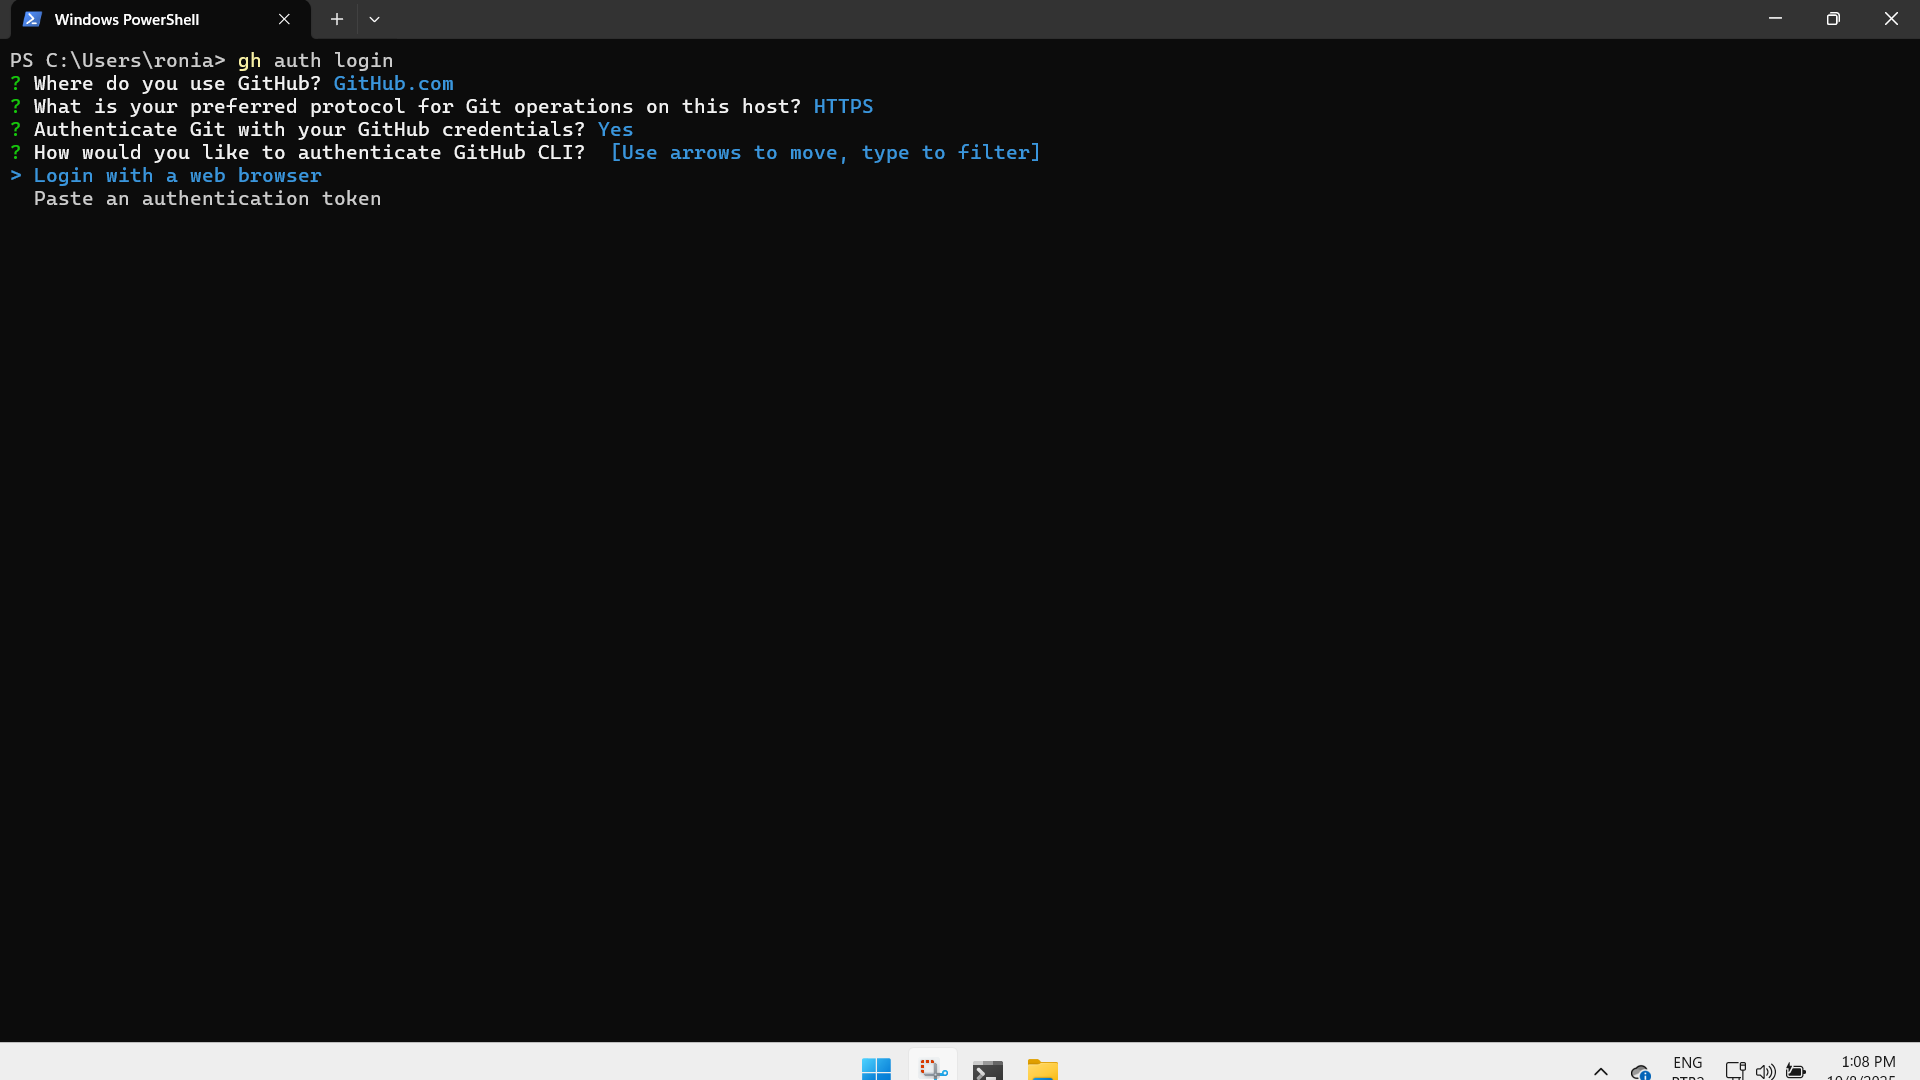
\includegraphics[width=0.9\textwidth]{./assets/images/13_3_gh_auth_login.png}
  \caption{Efetuando a autenticação com o GitHub-CLI - Passo 5.}
  \label{fig:gh_auth_login_4}
  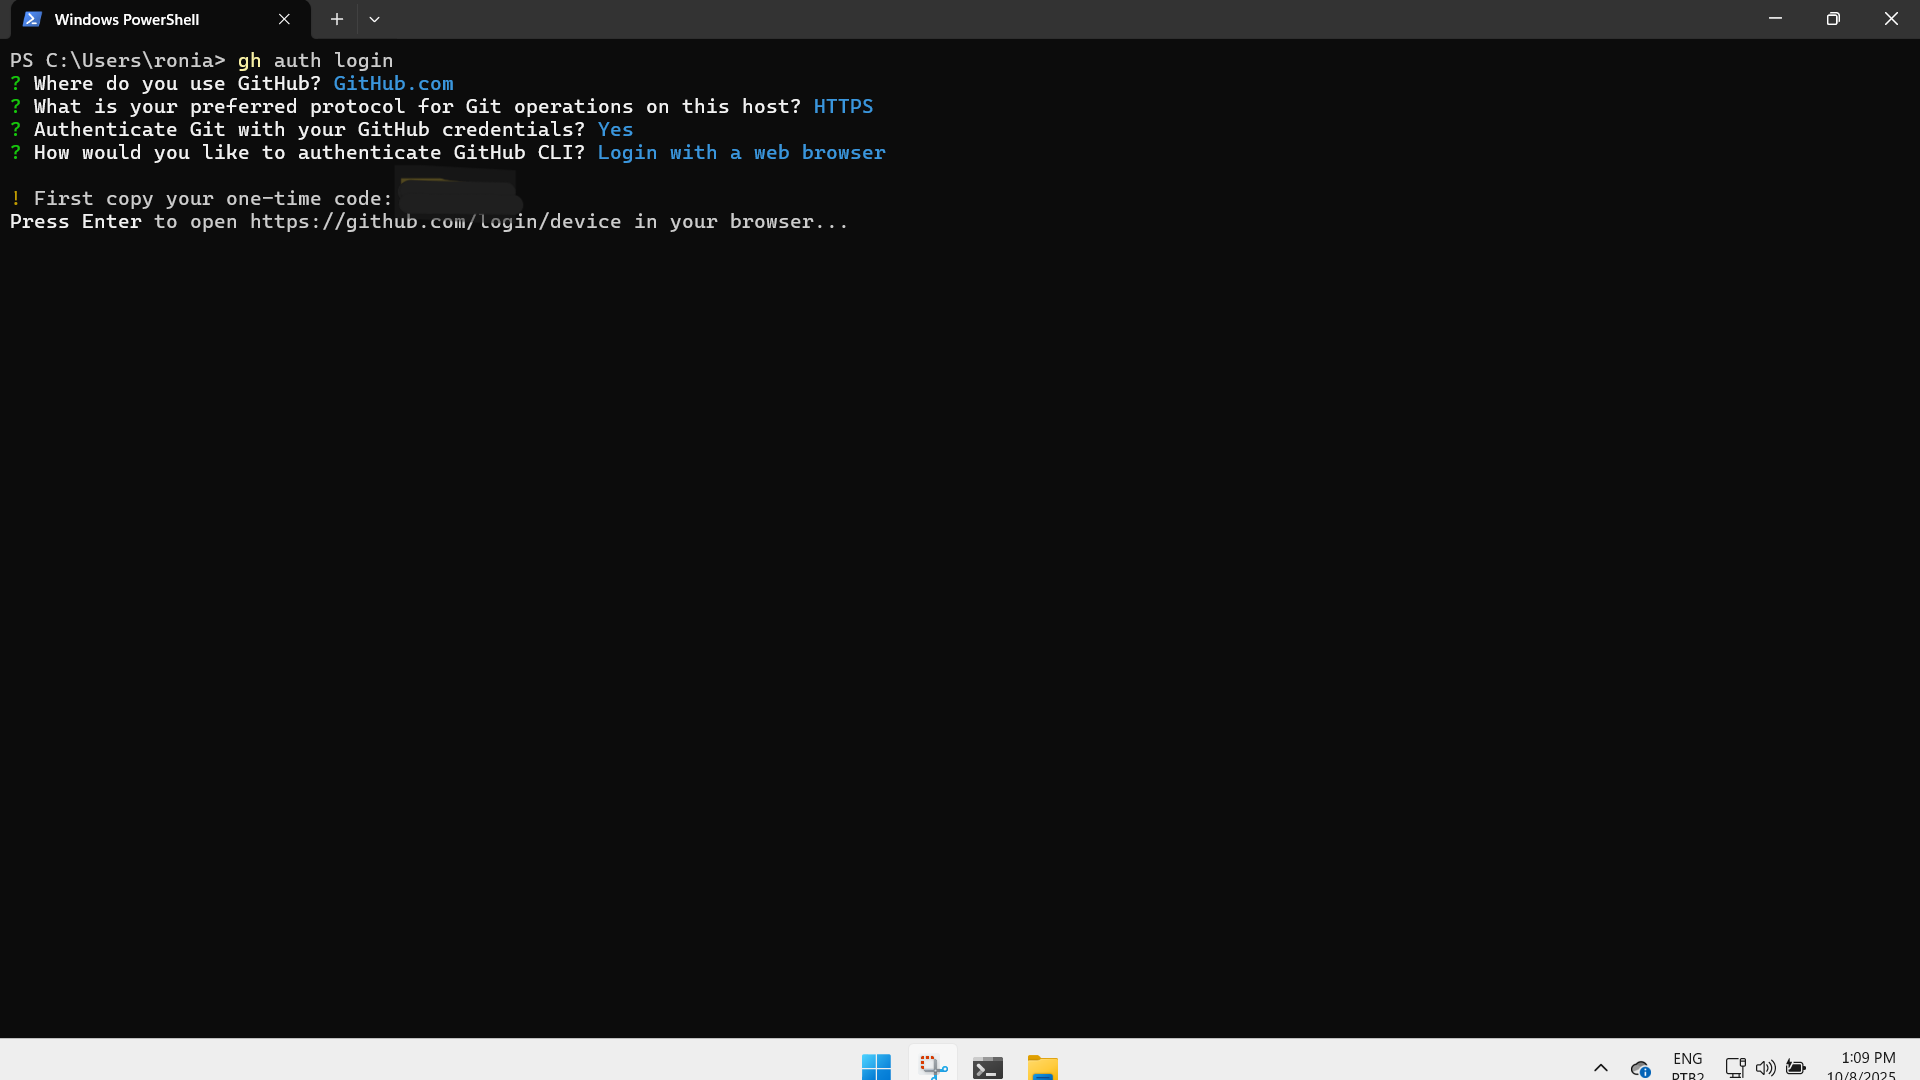
\includegraphics[width=0.9\textwidth]{./assets/images/13_4_gh_auth_login.png}
\end{figure}
\par
Após o passo 5 na Figura \ref{fig:gh_auth_login_4}, p.\pageref{fig:gh_auth_login_4}, será preciso copiar o código gerado abrir o navegador no link fornecido ou se precionar a tecla \texttt{Enter} abrirá o link automaticamente. Nessa tela será pedido que você se autentique e em seguida aparecerá o campo para digitar o código gerado e algumas permissões serão solicitadas.
\subsection{Configuração de usuário Git}
\begin{enumerate}
  \item Abra o Prompt de Comando ou PowerShell.
  \item Verifique a instalação do Git digitando:
  \begin{verbatim}
    git --version
  \end{verbatim}
  O comando deve retornar a versão do Git instalada.
  \item Configure seu nome de usuário com o comando:
  \begin{verbatim}
    git config --global user.name "Seu Nome"
  \end{verbatim}
  Substitua "Seu Nome" pelo nome que você deseja associar aos seus commits e pressione Enter.
  \item Verifique se o nome foi configurado corretamente com o comando:
  \begin{verbatim}
    git config --global user.name
  \end{verbatim}
  Pressione Enter.
  O comando deve retornar o nome que você configurou.
  \item Agora, configure seu e-mail com o comando:
  \begin{verbatim}
    git config --global user.email "Seu E-mail"
  \end{verbatim}
  Substitua "Seu E-mail" pelo e-mail que você deseja associar aos seus commits e pressione Enter.
  \item Verifique se o e-mail foi configurado corretamente com o comando:
  \begin{verbatim}
    git config --global user.email
  \end{verbatim}
  Pressione Enter.
  O comando deve retornar o e-mail que você configurou.
  \begin{figure}[H]
    \centering
    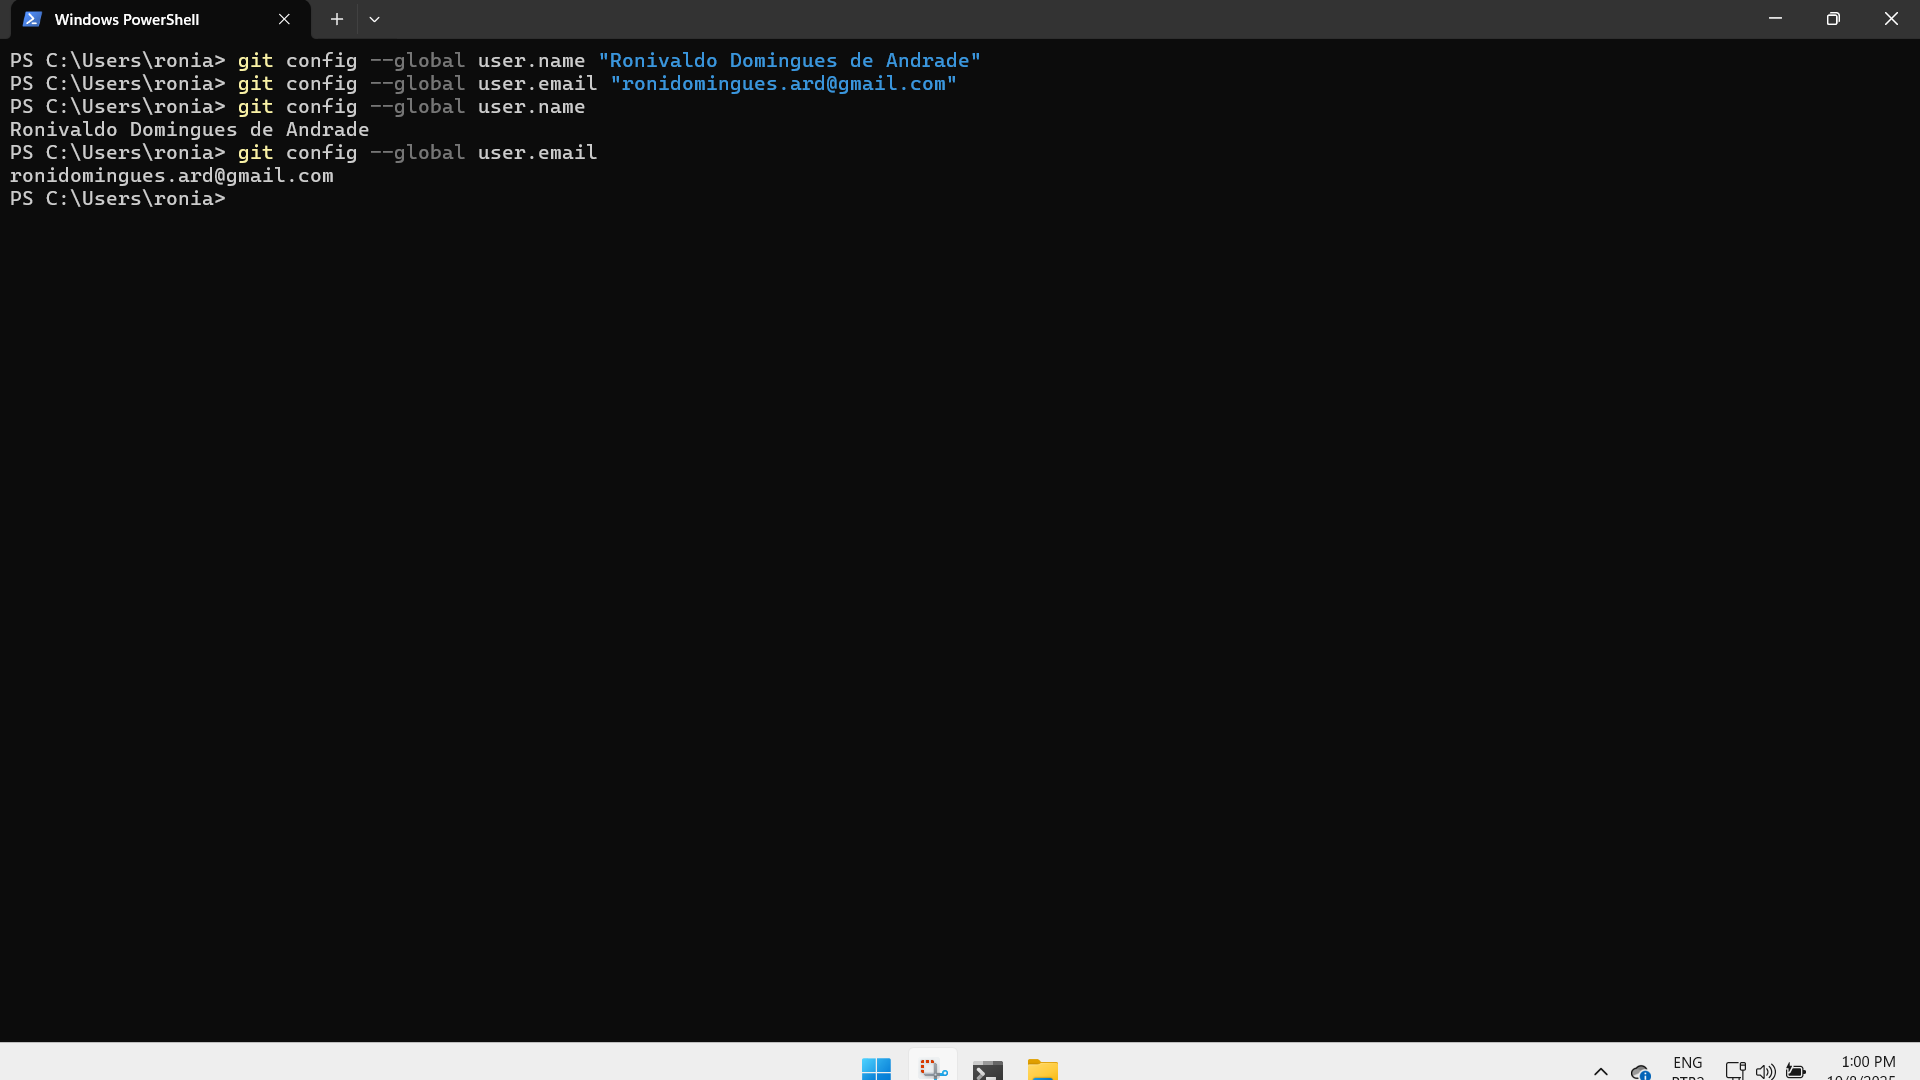
\includegraphics[width=0.9\textwidth]{./assets/images/14_git_base_config.png}
    \caption{Configurando o Git.}
    \label{fig:git_base_config}
  \end{figure}
\end{enumerate}
\par
\subsubsection{Autenticação usando PAT (Opcional)}
O uso da autenticação com Personal Access Token (PAT) no GitHub oferece maior segurança em comparação à utilização de senhas tradicionais. Isso porque o token pode ser revogado a qualquer momento diretamente nas configurações da conta, além de possuir um prazo de validade configurável no momento da criação.
Ademais, os PATs permitem definir escopos específicos de acesso, garantindo que o token tenha apenas as permissões necessárias para a operação desejada.
Se você optar por usar um Token de Acesso Pessoal (PAT) para autenticação, siga os passos abaixo:
\begin{enumerate}
  \item Acesse o link \url{https://github.com/settings/tokens} na sua conta do GitHub.
  \item Clique em "Generate new token (classic)".
  \item Marque escopos como:
  \begin{itemize}
    \item repo (para acesso completo a repositórios privados e públicos)
    \item  workflows (para gerenciar e visualizar GitHub Actions)
  \end{itemize}
  \item Clique em "Generate token" na parte inferior da página e copie o token gerado (ele não será mostrado novamente!).
  \item Agora, ao fazer um git push, quando o Git solicitar senha e usuario:
  \begin{itemize}
    \item Use seu nome de usuário do GitHub como usuário.
    \item Cole o token gerado como senha.
  \end{itemize}
  \item Você também pode salvar o token gerado no cache de credenciais do Git para evitar ter que digitá-lo toda vez que fizer push ou pull. Para isso, use o comando:
  \begin{verbatim}
    git config --global credential.helper store
  \end{verbatim}
  Com isso, na próxima vez que você digitar o token, ele será salvo no arquivo `~/.git-credentials` e usado automaticamente nas próximas operações.
\end{enumerate}
\par
\subsection{Configuração de Editor Padrão (Opcional)}
Você pode configurar o editor de texto padrão que será usado para escrever mensagens de commit. Por exemplo, para configurar o Visual Studio Code como editor padrão, use o comando:
\begin{verbatim}
  git config --global core.editor "code --wait"
\end{verbatim}
Substitua "code --wait" pelo comando do editor de sua preferência.
\par
\subsection{Configurar a branch padrão para 'main' (Opcional)}
Para configurar a branch padrão para 'main', use o comando:
\begin{verbatim}
  git config --global init.defaultBranch main
\end{verbatim}
Isso garantirá que novos repositórios criados localmente usem 'main' como a branch padrão. Caso não queira definir esse padrão é possivel mudar a branch individualmente para cada repositório com o comando:
\begin{verbatim}
  git branch -M main
\end{verbatim}
\par
Obs.: \textbf{A partir de outubro de 2020, o GitHub alterou o nome da branch padrão de "master" para "main" em novos repositórios. Portanto, é recomendável usar "main" como a branch padrão para novos projetos.}
\par
\section{Comandos Básicos do Git e GitHub-CLI}
Aqui estão alguns comandos básicos do Git e do GitHub-CLI que você deve conhecer para começar a trabalhar com repositórios no GitHub.
\par
\subsection{Comandos Básicos do Git}
\begin{itemize}
  \item \textbf{git init}: Inicializa um novo repositório Git local.
  \item \textbf{git clone <url>}: Clona um repositório remoto para o seu computador.
  \item \textbf{git status}: Exibe o status atual do repositório, mostrando arquivos modificados, não rastreados e prontos para commit.
  \item \textbf{git add <arquivo>}: Adiciona um arquivo específico ao estágio para commit.
  \item \textbf{git add .}: Adiciona todos os arquivos modificados ao estágio para commit.
  \item \textbf{git commit -m "mensagem"}: Cria um commit com uma mensagem descritiva.
  \item \textbf{git push}: Envia os commits locais para o repositório remoto.
  \item \textbf{git pull}: Puxa as alterações do repositório remoto para o repositório local.
  \item \textbf{git branch}: Lista todas as branches no repositório.
  \item \textbf{git checkout <branch>}: Muda para a branch especificada.
  \item \textbf{git branch -M <branch>}: Renomeia a branch atual para o nome especificado forçando a sobrescrita se a branch especificada já existir.
  \item \textbf{git branch -m <branch>}: Renomeia a branch atual para o nome especificado e falha se a branch especificada já existir.
  \item \textbf{git checkout -b <branch>}: Cria uma nova branch e muda para ela.
  \item \textbf{git branch -d <branch>}: Deleta a branch especificada.
  \item \textbf{git remote rm origin}: Remove o repositório remoto chamado "origin".
  \item \textbf{git remote add origin <url>}: Adiciona um repositório remoto com o nome "origin".
  \item \textbf{git remote -v}: Exibe os repositórios remotos configurados.
  \item \textbf{git merge <branch>}: Mescla a branch especificada na branch atual.
  \item \textbf{Veja mais comandos do Git na tabela \ref{tab:gitcommands}, p.\pageref{tab:gitcommands}.}
\end{itemize}
\par
\subsection{Comandos Básicos do GitHub-CLI}
\begin{itemize}
  \item \textbf{gh auth login}: Autentica o usuário no GitHub-CLI.
  \item \textbf{gh repo create <nome-do-repositorio>}: Cria um novo repositório no GitHub.
  \item \textbf{gh repo clone <nome-do-repositorio>}: Clona um repositório do GitHub para o seu computador.
  \item \textbf{gh issue create}: Cria uma nova issue no repositório atual.
  \item \textbf{gh pr create}: Cria um novo pull request.
  \item \textbf{gh pr checkout <numero-do-pr>}: Faz checkout de um pull request específico.
  \item \textbf{gh pr merge <numero-do-pr>}: Mescla um pull request específico.
  \item \textbf{gh repo view}: Exibe informações sobre o repositório atual.
  \item \textbf{gh gist create <arquivo>}: Cria um novo gist com o arquivo especificado.
  \item \textbf{Veja mais comandos do GitHub-CLI na tabela \ref{tab:githubcli_commands}, p.\pageref{tab:githubcli_commands}.}
\end{itemize}
\par